\section{Schaltkreise}
    Schaltkreise bestehen aus:
    \begin{itemize}
        \item Eingangsgatter
        \item Ausgänge
        \item Gatter
        \item Verbindungen (DAG)
    \end{itemize}
    \subsection{Beispiel}
        $x_1,x_2,x_3\in\{0,1\}$, $L=0^*10^*$\\
        \begin{tikzpicture}[label distance=2mm, minimum size=5mm]
            \node (x1) at (0,4) {$x_1$};
            \node (x2) at (0,2) {$x_2$};
            \node (x3) at (0,0) {$x_3$};

            \node[or gate IEC,draw,minimum size=1cm,logic gate IEC symbol align={center}] at ($(x2)+(8,0)$) (Or) {};

            \foreach \i in {1,2,3}
            {
                \node[not gate IEC, draw] at ($(x\i)+(1,1)$) (Not\i){};

                \node[and gate IEC, draw, minimum size=7mm,logic gate IEC symbol align={center}] at ($(x\i)+(4,0)$) (And\i){};

                \draw (x\i) -- coordinate (punt\i) (x\i -| Not\i.input);
                \draw (punt\i) node[branch] {} |- (Not\i.input);

                \draw (x\i) -- (And\i);
                \draw (And\i) -- ($(And\i)+(\i*0.5,0)$);

                \draw (Not\i.output) -- ($(Not\i.output)+(\i*0.5,0)$) coordinate (nn\i) ;
            }

            \draw ($(And1)+(0.5,0)$) |- (Or.input 1);
            \draw (And2) -- (Or);
            \draw ($(And3)+(3*0.5,0)$) |- (Or.input 2);

            \node[branch] at (nn2){};

            \draw (nn1) |- node[branch] {} (And2.input 1);
            \draw (nn1) |- (And3.input 1);
            \draw (nn2) |- (And1.input 1);
            \draw (nn2) |- (And3.input 2);
            \draw (nn3) |- (And1.input 2);
            \draw (nn3) |- node[branch] {} (And2.input 2);

            \draw (Or.output) -- ($(Or.output)+(0.5,0)$);
        \end{tikzpicture}
    \subsection{Anmerkungen, Schaltkreisfamilien}
        Mögliche Gatter: $AND,\ OR,\ MOD,\ MAJ,\ \dots$\\
        Für Spracherkennung: Schaltkreise für verschiedene Eingabelängen $\rightarrow$ Schaltkreisfamilien $\left(C_n\right)_{n\in\mathds{N}}$\\
        Bsp. leicht zu Familie erweiterbar.
        \subsubsection{Problematik}
            Schaltkreisfamilien können beispielsweise unäres Halteproblem entscheiden\\$\rightarrow$ Uniformität: Es existiert Algorithmus, der auf Eingabe $n$ den Schaltkreis $C_n$ berechnet. (z.B. $DLOGTIME$-uniform)
\section{Schaltkreise als Alternative zu Turingmaschinen}
    Komplexitätsmaße bei TM: Zeit, Platz
    Komplexitätsmaße bei Schaltkreisen: Größe, Tiefe, Gatter, Fan-in, Uniformität
    \subsection{Klassen}
        \subsubsection{NC}
            $NC^i$: polynomiell viele Gatter, $\mathcal{O}\left(\log^i(n)\right)$ Tiefe, Fan-in=2, Bool'sche Gatter\\
            $NC$: $\bigcup\limits_i NC^i$
        \subsubsection{AC}
            $AC^i$: wie $NC^i$ nur unbeschränkter Fan-in\\
            $AC:\ \bigcup\limits_i AC^i$
        \subsubsection{ACC}
            $ACC^i_k$: Wie $AC^i$ nur mit $MOD_k$-Gatter zusätzlich\\
            $ACC^i$: $\bigcup\limits_k ACC^i_k$
        \subsubsection{TC}
            $TC^i$: wie $AC^i$, ausschließlich $MAJ$-Gatter\\
            $TC:\ \bigcup\limits_i TC^i$
        \subsubsection{SAC}
            $SAC^i$: wie $AC^i$ nur $ODER$-Gatter haben unbeschränkten Fan-in\\
            $SAC$: $\bigcup\limits_i SAC^i$
        \subsubsection{CC}
            $CC^i$: Wie $AC^i$, ausschließlich $MOD$-Gatter\\
            $CC:$ $\bigcup\limits_i CC^i$
        \subsubsection{Anmerkung}
        \begin{itemize}
            \item Besonders interessant: $AC^0,\ ACC^0,\ TC^0,\ NC^1$
            \item $NC=AC=ACC=TC=SAC$
            \item $AC^{i-1}\subseteq NC^i$ (offensichtlich: Fan-in durch Tiefe)
        \end{itemize}
    \subsection{Satz}
        \textsc{Parity} nicht in $AC^0$ (Furst, Saxe, Sipser).
        \subsubsection{Anmerkung}
            Also $AC^0\subsetneq NC^1$.\\
            Offen:
            \begin{itemize}
                \item $TC^0\overset{?}{\subsetneq} NC^1$
                \item $ACC^0\overset{?}{\subsetneq} TC^0$
            \end{itemize}
    \subsection{Satz}
        Reguläre Sprachen (\textsc{Reg}) $\subseteq NC^1$
        \subsubsection{Beweis}
            Sei $L$ regulär, oBdA $L\subseteq\{0,1\}^*$\\
            Sei $|Synt(L)|=k$ und $\eta_L:\Sigmas\rightarrow Synt(L):w\mapsto [w]$\\
            nummeriere alle $m\in Synt(L)$ binär ($\lceil\log k\rceil$ Stellen): $\widehat{m}$
            Wir benötigen folgende Schaltkreise/Gatter:
            \begin{enumerate}[1)]
                \item $a\in\Sigma:\ a\mapsto\widehat{\eta_L(a)}$
                \item auf Eingabe $\widehat{m_1},\ \widehat{m_2}$, gib $\widehat{m_1m_2}$ aus
                \item gib 1 aus gdw. für Eingabe $\widehat{m}$ gilt $m\in\eta_L(L)$
            \end{enumerate}
            $\rightarrow$ Größe von 1),2),3) konstant in Wortlänge\\
            mit Baum $\log$-Tiefe kann Schaltkreisfamilie für $L$ angegeben werden.\\
            \scriptsize\vspace*{-3.7cm}\\
            \hspace*{10.5cm}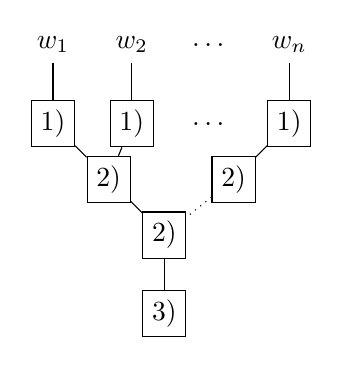
\begin{tikzpicture}
                [node distance=1cm]
                \node (w1) {$w_1$};
                \node (w2) [right of=w1] {$w_2$};
                \node (wi) [right of=w2] {\dots};
                \node (wn) [right of=wi] {$w_n$};
                \node[draw,rectangle] (11) [below of=w1] {1)};
                \node[draw,rectangle] (12) [right of=11] {1)};
                \node (1i) [right of=12] {\dots};
                \node[draw,rectangle] (1n) [right of=1i] {1)};

                \node[draw,rectangle] (21) [below right of=11] {2)} ;
                \node[draw,rectangle] (2n) [below left of=1n] {2)} ;

                \node[draw,rectangle] (2u) [below right of=21] {2)} ;

                \node[draw,rectangle] (3) [below of=2u] {3)};

                \foreach \i in {1,2,n}
                {
                    \draw (w\i) -- (1\i);
                }
                \draw (11) -- (21);
                \draw (12) -- (21);
                \draw (1n) -- (2n);
                \draw (21) -- (2u);
                \draw[dotted] (2n) -- (2u);
                \draw (2u) -- (3);
            \end{tikzpicture}
            \normalsize
    \subsection{Satz}
        \textsc{Reg} ist $NC^1$ vollständig (beweisen wir hier nicht)
    \subsection{Satz von Buss}
        Auswertungsproblem für Bool'sche Formeln ist $NC^1$-vollständig.
    \subsection{Satz}
        $VPL\subseteq NC^1$ (Dymond ``input-driven PDA'') und $NC^1$-vollständig, da \textsc{Reg}$\subseteq VPL$
    \subsection{Satz}
        $CFL$ ist $SAC^1$-vollständig.
    \subsection{Satz}
        $FO[arb]=AC^0$
        \subsubsection{Beweis $\subseteq$}
            $\exists x\varphi(x)\rightarrow \bigvee\limits_{i=1}^n \varphi(i)$\\
            $\forall x\varphi(x)\rightarrow \bigwedge\limits_{i=1}^n \varphi(i)$\\
            $Q_0i,\ Q_1i\rightarrow$ Eingang $x_i$ bzw. $\bar{x_i}$\\
            $R(i_1,\dots,i_k)\rightarrow$ 0 bzw. 1, je nach Wert von $(i_1,\dots,i_k)$
    \subsection{weitere Sätze}
        \begin{itemize}
            \item $MOD_q[arb]=CC^0_q$
            \item $FO+MOD_q[arb]=ACC_q^0$
            \item $DLOGTIME$-uniform $AC^0=FO[+,\times]$
        \end{itemize}

